\section{RAGChecker Framework}

% \pfliu{before diving into our RAGChecker, We need a subsection or even section to introduce some basics or preliminaries about (a) RAG setting, for example, what are retrieved contexts, generator, groundtruth answer. (b) existing typical evaluation methods for RAG }

\paragraph{Formulation} Define a modular RAG system as $\text{RAG} = \{\text{R}, \text{G}\}$, where $\text{R}$ is the retriever and $\text{G}$ is the generator. Given a query $q$ and documents $D$, it first retrieves top-$k$ relevant context $\{\text{chunk}_j\}=\text{R}(q, D, k)$, and then generates a response $\text{Res} = \text{G}(\{\text{chunk}_j\}, q)$. For simplicity, we can also represent the overall RAG generation process as $\text{Res} = \text{RAG}(q, D)$.

\paragraph{Design Principle} Given the compositional nature of RAG, we observe there are two major personae using a RAG evaluation framework. The first persona is a user that care about the overall performance of RAGs, and might choose a system with the best cost-performance. Such a persona prefers a single value metric to compare and rank among RAG systems against a benchmark. The second persona is a developer that focuses on improving a RAG system with the need to identify causes of mistakes and potential rooms for improvements. Causes of mistakes can be classified into (1) retrieval errors, where the retriever fails to return complete and relevant context, and (2) generator errors, where the model struggles to effectively leverage contextual information or generates hallucinated content.

Consequently, metrics that reveal error causes should be different from those for overall performance, in the sense that error causes are module-specific or even reflected only by a certain behavior of a module. To help both personae to assess RAG performance, we design RAGChecker, a evaluation framework of RAG systems that consists of a benchmark with rich annotations and a set of diversely-purposed fine-grained metrics.

\subsection{Benchmark annotations}

We prepare each sample in our benchmark dataset in the format of a tuple $\left< q, D, \text{GT-A}\right>$ representing query, documents, and groundtruth answer, where query is the input question to a RAG system, documents form the database providing possible context and are processed into chunks with the same number of tokens, and groundtruth answer is a complete and correct answer for the input question. Specific curation process is described in Sec.~\ref{appendix:benchmark}.

\subsection{Fine-grained evaluation with claim entailment}

As illustrated in Fig.~\ref{fig:metrics}, a response generated by a RAG system might contain a mixture of correct (\hollowcircle) and incorrect claims (\crossmark), while missing some in-groundtruth claims (\hollowtriangle). In this sense, evaluating responses at a finer grain is crucial to comprehensively assess the quality of an answer. For this purpose, we introduce two components: (1) a text-to-claim extractor that breaks a given text $T$ into a set of claims $\{C_i\}$, and (2) a claim-entailment checker to determine whether a given claim $c$ can entail ($\in$) a reference text $Ref$ or not($\notin$)

\subsection{RAGChecker metrics}

With the annotations and components specified, we introduce the metrics in the following subsections. The design philosophy of all metrics is to obtain claim entailment labels ($\in$ or $\notin$) given any to-evaluate text $T$ and reference text $Ref$, where $T$ and $Ref$ can be model response, groundtruth answer, or retrieved chunks.

For a RAG user, we design metrics to compare the performance among RAG systems, including a single-value F1 score as a overall metric. For a RAG developer, on the other hand, we propose two sets of modular metrics for the retriever and the generator in a RAG system respectively, that are supposed to be able to decomposite the system and diagnose the source of errors. In the rest of this section, we will first introduce the overall metrics, and then go over metrics for retriever and generator separately.


\begin{figure}[ht]
    \centering
    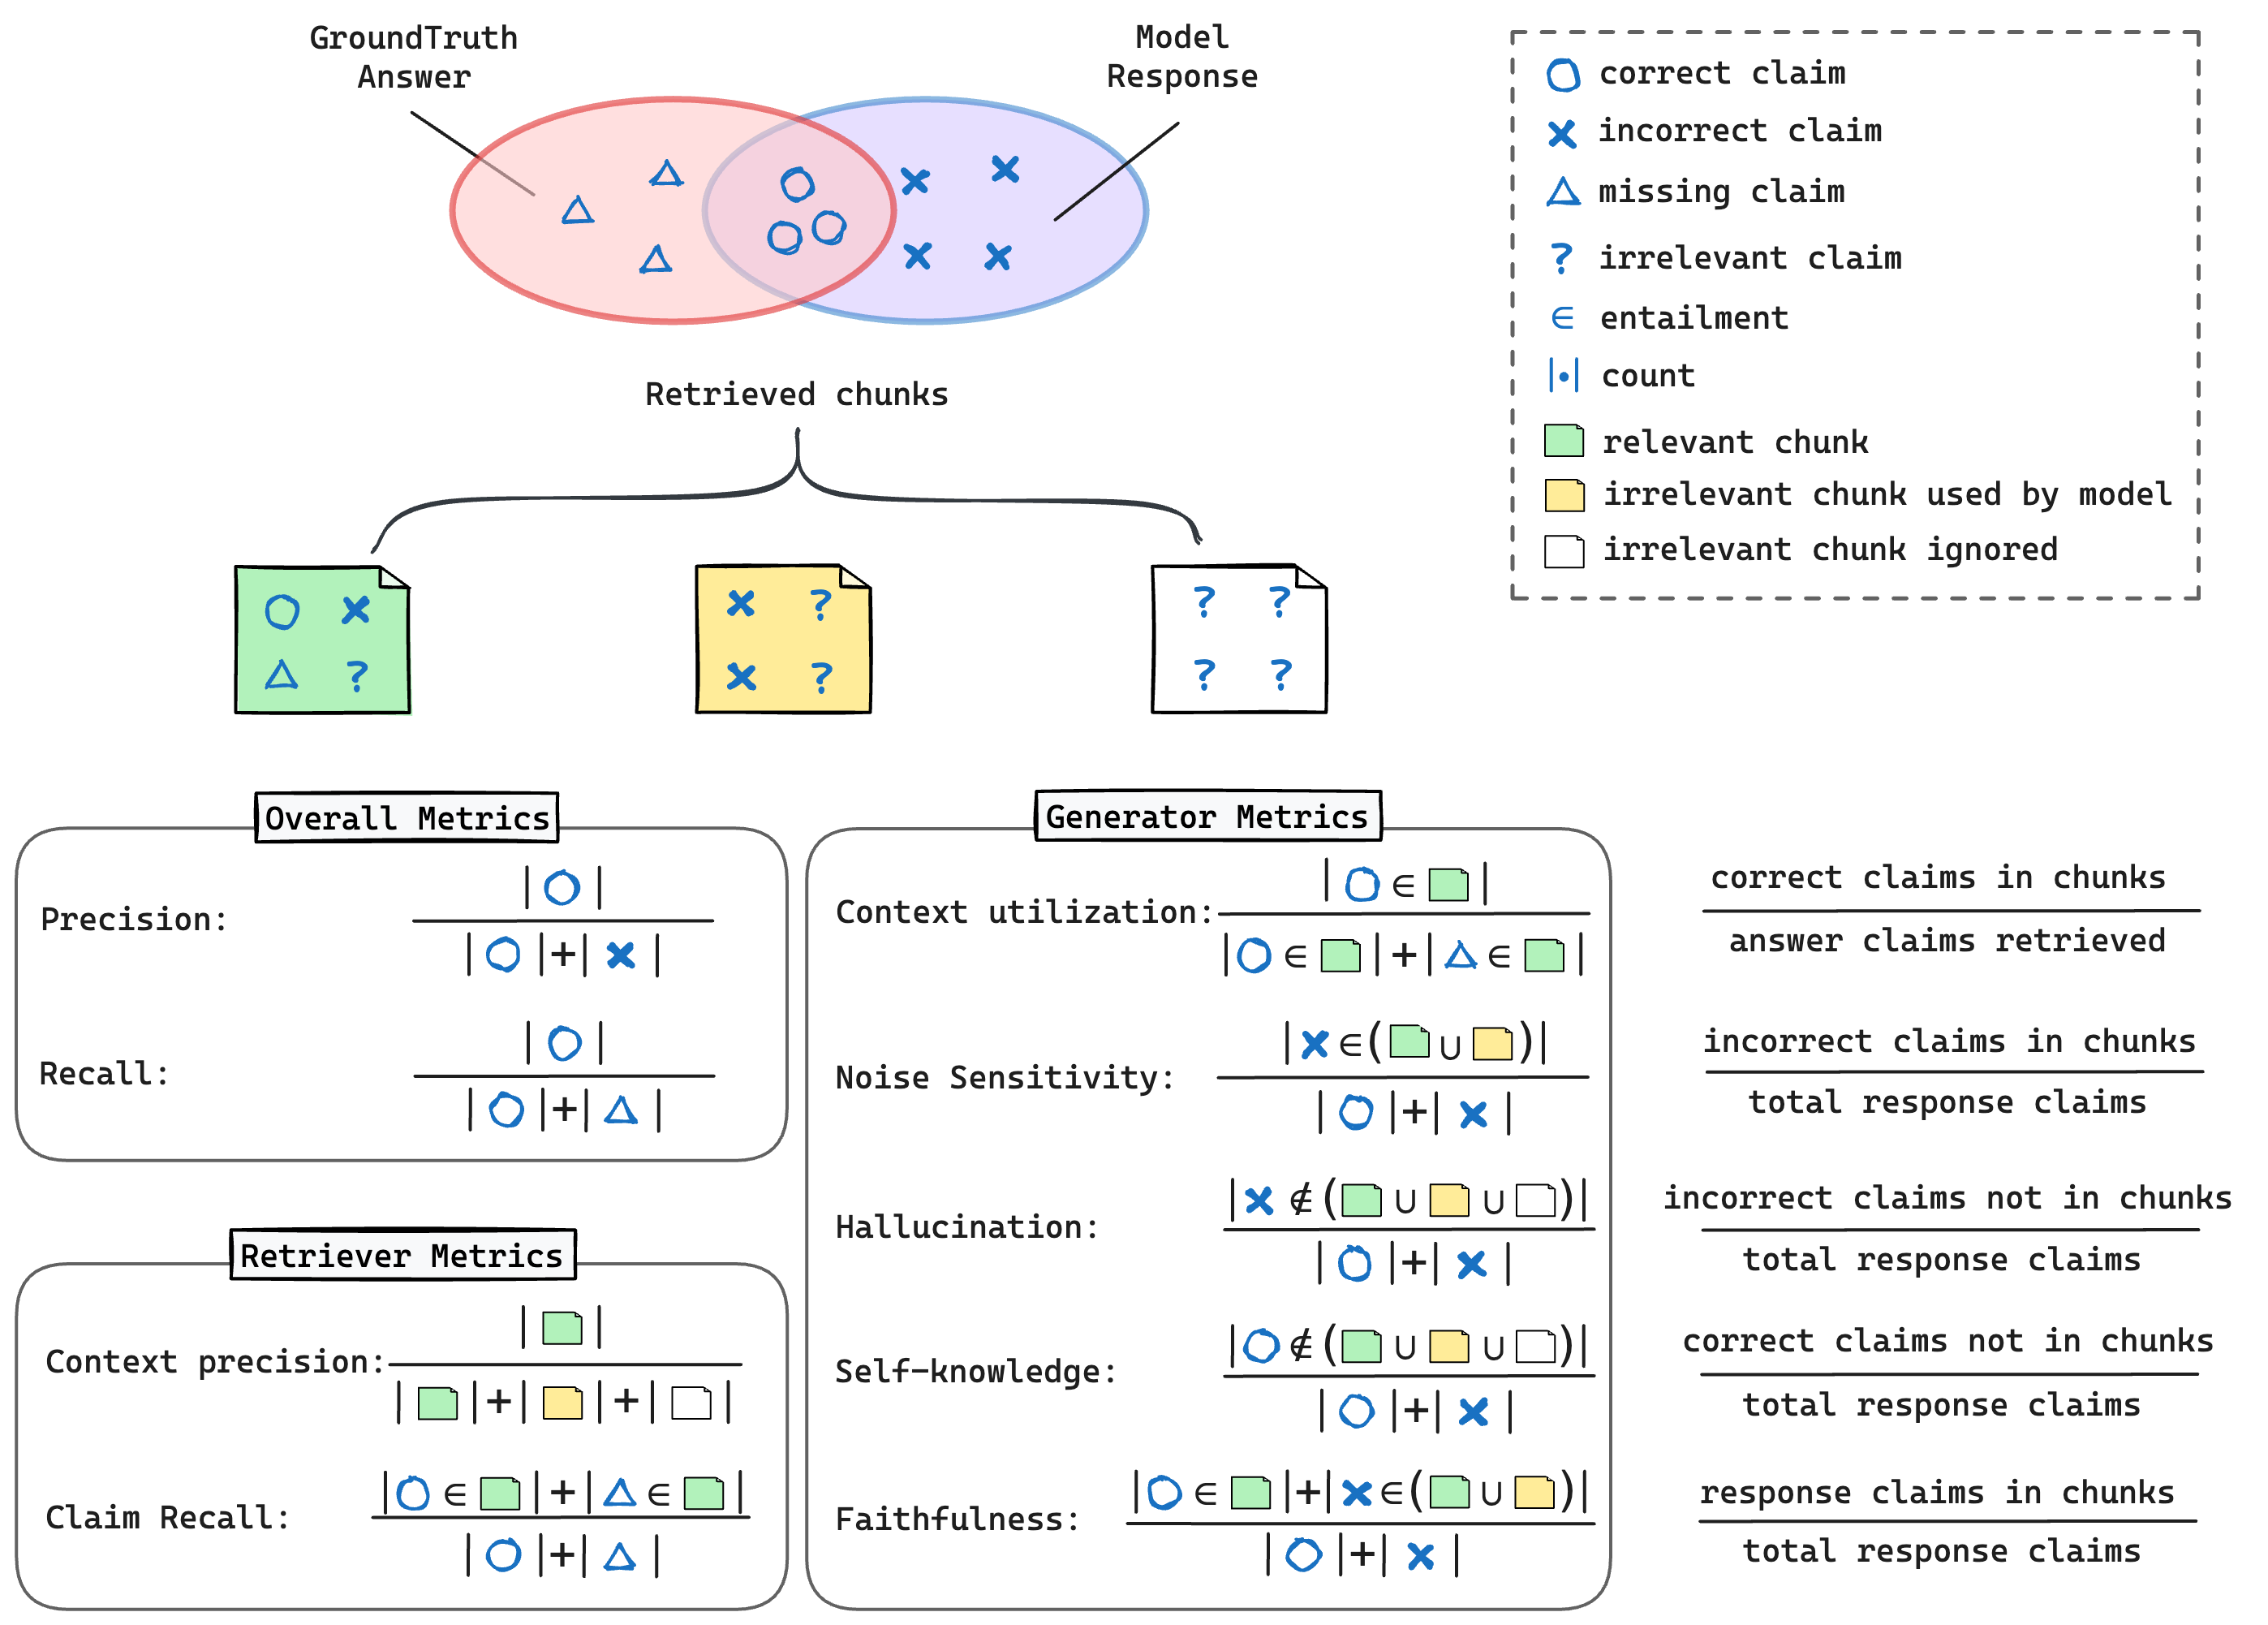
\includegraphics[width=0.9\textwidth]{figures/ragchecker_metrics.png}
    \caption{Illustration of our proposed metrics.}
    \label{fig:metrics}
\end{figure}

\subsubsection{Overall metrics}

To assess the overall response quality of a RAG system from a user’s perspective, we can compute the precision and recall at claim level for each model generated response against its paired groundtruth answer. Specifically, we first extract claims from a model response $m$ and a groundtruth answer $gt$ as $\{C^{(m)}_i\}$ and $\{C^{(gt)}_i\}$, respectively. Then compute the correct claims in the response as $\{c^{(m)}_i | c^{(m)}_i \in gt\}$ and correct claims in ground truth answer as $\{c^{(gt)}_i | c^{(gt)}_i \in m\}$. Then we compute the response \textbf{precision} as the ratio of correct claims in the response and response \textbf{recall} as the ratio of correct claims in the ground truth answer. Further, the harmonic average of precision and recall gives the \textbf{F1} score, as the overall performance metric.

\subsubsection{Retriever metrics}
\label{sec:retriever_metrics}
Ideally, a perfect retriever returns precisely all claims needed to generate the groundtruth answer. Completeness-wise, we can measure how many claims made in the groundtruth answer are covered by retrieved chunks. Formally, with retrieved chunks as the reference text, we compute \textbf{claim recall} as the ratio of ground truth answer claims entailed in the retrieved chunks where such claims are defined as $\{c^{(gt)}_i | c^{(gt)}_i \in \{\text{chunk}_j\}\}$.


Differently, we define the retriever precision at chunk-level instead of claim-level. A retrieved chunk is called \textit{relevant chunk} ($\text{r-chunk}$, shown by green color in Fig.~\ref{fig:metrics}), if any groundtruth claim is entailed in it. In other words, $\text{chunk}_j$ is a relevant chunk if $\exists i ~s.t.~ c^{(gt)}_i\in \text{chunk}_j$. The rest retrieved chunks are called \textit{irrelevant chunk} ($\text{irr-chunk}$, shown by yellow or white color in Fig.~\ref{fig:metrics}). The \textbf{context precision} is defined as $|\{\text{r-chunk}\}|/k$, where $k$ is the number of all retrieved chunks. This design choice is made because of the fix-size chunking strategy adopted in practice: the entire database is split into chunks of the same length, therefore it is possible that a chunk may contain relevant claims and irrelevant or misleading information at the same time. As a result, the best possible retriever can only achieve a claim-level precision score lower than 100\%, and the actual upper-bound varies depending on the actual text distribution in $D$ and chunking strategy.


\subsubsection{Generator metrics}

Given $k$ retrieved chunks (possibly as a mixture of relevant and irrelevant information), a perfect generator would identify and include all groundtruth-relevant claims, and ignore any that are not. Because the generator’s results depends on retrieved chunks, we provide in total six metrics characterizing different aspects of its performance.

Given a model response $m$ and its claims $\{C^{(m)}_i\}$, we first check how many of the claims are entailed in the retrieved content. This number over all response claims is called \textbf{faithfulness}, as it describes how faithful the generator is to the provided context, thus the higher the better.

Next, we define incorrect claims in response as $\{c^{(m)}_i | c^{(m)}_i \notin gt\}$. These incorrect claims can be further classified into three types. If an incorrect claim is not entailed in any retrieved chunk, then this claim is generated by the generator itself, meaning it is a \textbf{hallucination}. By definition, other incorrect claims are entailed by a retrieved chunk. As discussed in Sec.~\ref{sec:retriever_metrics}, a chunk may come with a mixture of relevant and irrelevant information, and if an incorrect response claim is entailed to such a chunk, it means that the generator is \textbf{sensitive to the noise in relevant chunks}. Similarly, if an incorrect claim is entailed to a chunk with only irrelevant information , then it means the generator is \textbf{sensitive to the noise in irrelevant chunks}. For simplicity, we group the two metrics into \textbf{noise sensitivity} in Fig.~\ref{fig:metrics}. All three metrics are computed as the ratio of corresponding claims over all the response claims and expected to be low for a good generator.

Finally, we check the source of all correct claims, i.e. with $\{c^{(m)}_i | c^{(m)}_i \in gt\}$. A correct claim not entailed to any chunk is based on generator’s \textbf{self-knowledge}, it reflects how many correct claims are generated on its own. With the expectation that the generator in a RAG system should fully depend on retrieved context only, a lower self-knowledge score is better. On the other hand, we define \textbf{context utilization} to check how much retrieved knowledge is picked up by the generator where retrieved knowledge is measured by the number of ground truth answer claims entailed in retrieved chunks. Obviously, A high context utilization is preferred.


%precision:
%$|\{c^{(m)}_i | c^{(m)}_i \in gt\}|/|\{C^{(m)}_i\}|$
%recall:
%$|\{c^{(gt)}_i | c^{(gt)}_i \in m\}|/|\{C^{(gt)}_i\}|$

%claim recall:
%$|\{c^{(gt)}_i | c^{(gt)}_i \in \text{chunk}_j\}|/|\{C^{(gt)}_i\}|$

%faithfulness:
%(|\{c^{(gt)}_i |c^{(gt)}_i \in m\& c^{(gt)}_i\in\{\text{r-chunk}\}\}| + |\{c^{(m)}_i |c^{(m)}_i \notin gt\& c^{(m)}_i\in\{\text{chunk}\}\}|)/|\{C^{(m)}_i\}|
%hallucination:
%$|\{c^{(m)}_i |c^{(m)}_i \notin gt\& c^{(m)}_i\notin\{\text{chunk}\}\}|/|\{C^{(m)}_i\}|$
%relevant noise sensitivity:
%$|\{c^{(m)}_i |c^{(m)}_i \notin gt\& c^{(m)}_i\in\{\text{r-chunk}\}\}|/|\{C^{(m)}_i\}|$. 
%irrelevant noise sensitivity:
%$|\{c^{(m)}_i |c^{(m)}_i \notin gt\& c^{(m)}_i\in\{\text{irr-chunk}\}\}|/|\{C^{(m)}_i\}|$.
%self-knowledge:
%$|\{c^{(m)}_i |c^{(m)}_i \in gt \&c^{(m)}_i\notin\{\text{chunk}\}\}|/|\{C^{(m)}_i\}|$
%context utilization:
%$|\{c^{(gt)}_i |c^{(gt)}_i \in m\& c^{(gt)}_i\in\{\text{r-chunk}\}\}|/|\{C^{(gt)}_i\in\{\text{chunk}\}\}|$